%&latex
%
\providecommand{\main}{../..}
\documentclass[../../main.tex]{subfiles}

\begin{document}

\section{Critical Behaviours and Scaling Laws}
\lesson{22}{29/04/20}

In the last section, we were able to finally describe a \textbf{phase-transition} , by analysing the Ising Model in the mean field approximation in $d > 1$. Mathematically, we observed how the \textbf{spontaneous magnetization} $M(K, h)$,\marginpar{Power laws} when $K$ is chosen in the proximity of the \textit{critical parameter} $K_c$ needed for the phase-transition, is described by a \textbf{power law} (\ref{eqn:mean-field-MS}).

\medskip

This happens to be a very general kind of behaviour, proper of \textbf{not only} \textbf{mean field} models.
Scaling laws such as (\ref{eqn:mean-field-MS}) were originally formulated from empirical evidence, and then given a theoretical foundation in the 1960s by Widom, Kadanoff and Kenneth Wilson, leading to the field of \textbf{renormalization group theory}. In this framework, all critical phenomena can be treated on equal ground, and general results can be mathematically proven. 

\medskip

The importance of scaling laws, and especially the values of their \textit{critical exponents} (such as $\beta$ for the IM) resides in their \textbf{universality}, i.e. in the fact that they are \textit{largely independent} on the \q{model's details}. In other words, the very same scaling law can describe two systems that - from the outside - seem completely different - but that share some fundamental characteristic (e.g. symmetry). 

\medskip

So, let's continue using the Ising Model in the mean field approximation as a \textit{concrete} example, and let's focus on deriving and understanding scaling laws for various quantities of interest.

\subsection{Spontaneous magnetization}
We start with (re)deriving the power law for the \textbf{spontaneous magnetization}. Recall the expression for the variational free energy (\ref{eqn:FV-uniform}):
\begin{align}\label{eqn:FV-uniform2}
    \beta \frac{F_V(m,K,h)}{N} = - K d m^2 + \frac{1+m}{2} \ln \frac{1+m}{2} + \frac{1-m}{2} \ln \frac{1-m}{2} - hm   
\end{align}
$F_V$ is closest to the \textit{true} \q{unapproximated} free energy $F$ when it's minimum:
\begin{align}\label{eqn:minimizing-eq}
    \pdv{m} F_V(m, K, h) \overset{!}{=} 0 \underset{(\ref{eqn:uniform-variational-eq})}{\Rightarrow}  m(h,K) = \tanh(2d K m + h)
\end{align} 
Let's solve (\ref{eqn:minimizing-eq}) for $h$ and expand\footnote{For notational simplicity, we do not denote with $M$ the value of $m$ that solves (\ref{eqn:minimizing-eq}), as was instead done in the previous section.} for $m \approx 0$, which holds near the critical temperature $T \approx T_c$:
\begin{align}\nonumber
    h &= -2dKm + \tanh^{-1}m  \underset{(\ref{eqn:inv_tanh})}{=} -2dKm + \frac{1}{2} \ln \frac{1+m}{1-m} \underset{(\ref{eqn:tanh})}{=} -2dKm + \frac{1}{2}[\ln(1+m) - \ln(1-m)] =\\ \nonumber
    &= -2dKm +\frac{1}{2}\left[m-\cancel{\frac{m^2}{2}}+\frac{m^3}{3}-\bcancel{\frac{m^4}{4}}+\frac{m^5}{5}+\dots  - \left(-m -\cancel{\frac{m^2}{2}} -\frac{m^3}{3} -\bcancel{\frac{m^4}{4} }-\frac{m^5}{5} + \dots    \right) \right] =\\
    &= m(1-2dK) + \frac{m^3}{3} + \frac{m^5}{5} + \dots  \label{eqn:h-eq} 
\end{align}
When $\textcolor{Blue}{h=0}$\marginpar{1. $h=0$} and $K \geq K_c = 1/2d$, then\footnote{Consider fig. \ref{fig:phase-diagram-uniform}, pag. \pageref{fig:phase-diagram-uniform}. When $h=0$, we are \q{moving} along a horizontal line, encountering the singularity at $K = K_c$.} $1-2dK < 0$. We already know that the solution $m=0$ is a local \textit{maximum} of $F_V$, and the minima are given by the other \textit{two} solutions. Dividing by $m$ and rearranging leads to:
\begin{align*}
    (2dK-1) = \frac{m^2}{3} + \frac{m^4}{5} + \dots \Rightarrow  m^2 = 3(2dK - 1) - \frac{m^4}{5} + \dots
\end{align*}
If $(2dK - 1)$ is of order $O(m^2)$, then $m^4$ is of order $O[(2dK-1)^2]$, and so:
\begin{align*}
    m^2 = 3(2dK-1) + O[(2dK-1)^2]
\end{align*}
And substituting $K_c = 1/2d$:
\begin{align}\label{eqn:msquareK}
    m^2 = 3\left(\frac{K}{K_c}-1 \right) + \dots = 3 \frac{K-K_c}{K_c} + O\left(\left[\frac{K-K_c}{K_c} \right]^2\right) 
\end{align}
Then, using $K=J/k_B T$ and $K_c = J/k_B T_c$ leads to the equivalent relation in terms of temperatures:
\begin{align*}
    m^2 &= 3 \frac{\sfrac{J}{k_BT} - \sfrac{J}{k_B T_C}}{\sfrac{J}{k_B T_C}} +\dots = 3 \frac{\sfrac{1}{T} - \sfrac{1}{T_c}}{\sfrac{1}{T_c}} +\dots = 3\left(\frac{T_c - T}{T} \right) \underbrace{\frac{\textcolor{Red}{T}}{\textcolor{Red}{T_c}}}_{\approx 1}  + \dots =\\ 
    &= 3 \underbrace{\frac{T_c - T}{T_c}}_{-t} + O\left(\left[\frac{T_c - T}{T_c} \right]^2\right)  = 3 |t| + O(t^2) \qquad t \equiv \frac{T-T_c}{T_c} 
\end{align*} 
Taking the square root leads to the power law for the magnetization:
\begin{align}\label{eqn:m-power-law-h0}
    m = \sqrt{3} |t|^\beta \theta(-t) \qquad \beta = \frac{1}{2} 
\end{align}
Here, the Heaviside function $\theta(-t)$ ensures that $m=0$ for $T > T_c$.

\medskip

Let's now consider (\ref{eqn:h-eq}) in the case $\textcolor{Blue}{h \neq 0}$ \marginpar{2. $h\neq 0$}. To \q{see} the phase-transition, we fix\footnote{Referring to fig. \ref{fig:phase-diagram-uniform}, \pageref{fig:phase-diagram-uniform}, we are \q{moving} along a vertical line with $K = K_c$} any $K \geq K_c$, for example (and for simplicity) $K=K_c = 1/2d$. In this case, $1-2dK = 0$ and the linear term in (\ref{eqn:h-eq}) vanishes:
\begin{align}\label{eqn:m-power-law-h}
    h = \frac{m^3}{3} + \frac{m^5}{5} + \dots \underset{m\sim 0}{=} \frac{m}{3} |m|^{\delta - 1} \qquad \delta=3
\end{align}
After collecting a $m$, all the powers are even, and so we can insert a modulus\footnote{This is done so that the resulting expression is meaningful for any real $\delta$. Otherwise, we would have problems when a negative $m$ is elevated to a fractional exponent, such as $1/2$, leading to results that are complex - meaning that we would have to add more specifications. The notation $m|m|^{\delta-1}$ naturally solves this kind of trouble.}. The exponent of the leading order is then $\delta=3$.

\subsection{Susceptibility (at $h=0$)}
Near criticality, also the susceptibility $\chi$, measuring \q{how much} the system reacts to a change in the external field, obeys a power law.

\medskip

Recall that the susceptibility $\chi$ is defined as:
\begin{align*}
    \chi^{-1} \underset{(\ref{eqn:susceptibility})}{\equiv} \pdv{h}{m}   
\end{align*}
Using the expression (\ref{eqn:h-eq}) for $h$ and expanding around $m = 0$ we get:
\begin{align*}
    \chi^{-1} = \pdv{h}{m} \underset{(\ref{eqn:h-eq})}{=}  -2dK + \frac{1}{1-m^2}  = 1 - 2dK + m^2 + O(m^4)
\end{align*}
And using (\ref{eqn:m-power-law-h0}) to compute $m^2$ we arrive to:
\begin{align*}
    \chi^{-1} \Big|_{h=0} \underset{(\ref{eqn:m-power-law-h0})}{=} \begin{cases}
        1 - 2 d K = \frac{K_c-K}{K_c} = \frac{T-T_c}{T} = t+ O(t^2) & T > T_c \> (m=0)\\  
        1 - 2 dK + m^2 = \frac{K_c-K}{K_c} + 3\frac{K-K_c}{K_c} = 2|t| + O(t^2) & T<T_c 
    \end{cases}
\end{align*}
Taking the reciprocal we finally get the power law for $\chi$:
\begin{align}\label{eqn:susceptibility-power-law}
    \chi = A_\pm |t|^{-\gamma} \qquad \gamma = 1
\end{align}
with $A_+ = 1$ for $t > 0$, and $A_- = 1/2$ for $t<0$. A plot of $\chi(T)$ is shown in fig. \ref{fig:chi-cv}, and shows how it diverges for $T \to T_c$. In other words, near criticality, a small change in $h$ produces a \textit{infinite} change of $m$ - i.e. the system is \textit{globally} sensitive to the external field.

\medskip

This kind of \textit{global reaction} to \textit{small changes} is a defining characteristic of complex systems, such as living organisms - with the difference that they seems to \q{always} be near criticality. One example is a bird flock - which can be hundreds of meters in size - reacting almost instantaneously to a predator (very small in comparison). 

\subsection{Specific heat (at $h=0$)}
Another quantity of interest is the \textbf{specific heat}, defined as:
\begin{align*}
    C \equiv \pdv{\langle \mathcal{H} \rangle}{T}
\end{align*} 
Recalling that:
\begin{align*}
    -\langle \mathcal{H} \rangle = \pdv{\beta} \ln Z
\end{align*}
we get:
\begin{align*}
    C = \pdv{\langle \mathcal{H} \rangle}{T} = -\pdv{\beta}{T} \pdv[2]{\beta} \ln Z = \frac{1}{k_B T^2} \pdv[2]{\beta} (-\beta F) 
\end{align*}
The specific heat \textit{per node} at $h=0$ is then:
\begin{align*}
    c &= \frac{C}{N} \underset{(\ref{eqn:FV-uniform2})}{=} -k_B \beta^2 \pdv[2]{\beta} [-K d m^2 + \frac{1+m}{2}\ln\frac{1+m}{2} + \frac{1-m}{2}\ln\frac{1-m}{2}] =\\
    &\underset{\mathclap{\substack{m\approx0\\(\ref{eqn:free-energy-expansion-h0})}}}{=} \> -k_B \beta^2 \pdv[2]{\beta} \left(\frac{1-2dK}{2} m^2 + \frac{m^4}{12} + O(m^6)\right) =\\
    &= -k_B \beta^2 \pdv[2]{\beta} \left(-\frac{1}{2}\left(\frac{K}{K_c} -1 \right)m^2 + \frac{m^4}{12} + O(m^6) \right)
\end{align*}
For $K < K_c$ ($T > T_c$), $m\equiv 0$ (\ref{eqn:m-power-law-h0}) and so $c=0$. Otherwise, for $K > K_c$ ($T < T_c$), using (\ref{eqn:msquareK}) leads to:
\begin{align*}
    c &= -k_B \beta^2 \pdv[2]{\beta} \left(-\frac{3}{2}\left(\frac{K}{K_c}-1 \right)^2 + \frac{9}{12}\left(\frac{K}{K_c} -1\right)^2 + O\left(\left[\frac{K}{K_c}-1 \right]^3\right) \right) =\\
    &= \cancel{-}k_B \beta^2 \pdv[2]{\beta} \left(\cancel{-}\frac{3}{4} \left[\frac{K}{K_c} - 1 \right]^2 + \dots \right) \approx \frac{3}{4}  k_B \beta^2 \pdv{\beta} \frac{2J}{K_c}  \left(\frac{K}{K_c}-1 \right) = \frac{3}{2} k_B \frac{\overbrace{J \beta^2}^{K^2}}{K_c} =\\
    &\underset{K \approx K_c}{=} \frac{3}{2}k_B 
\end{align*}

In summary: \marginpar{\danger In the slides it is $\sfrac{3}{4}$ instead.}%TODO In the slides it is 3/4. Why? %https://courses.physics.ucsd.edu/2010/Spring/physics210a/LECTURES/CH07.pdf See 7.71
\begin{align}\label{eqn:specific-heat-power-law}
    c(T) = \begin{cases}
        0 & T > T_c\\
        \frac{3}{2}k_B & T<T_c 
    \end{cases} \propto |t|^{-\alpha} \qquad \alpha = 0 
\end{align} 
Here we would expect $C(T)$ to diverge near the critical temperature, with some exponent $\alpha$, but this does not happen in the mean-field approximation (and so we say $\alpha=0$). However, in Onsanger's exact solution for the $d=2$ case, $c(T)$ diverges logarithmically. 

\begin{appr}\textbf{Mean field and specific heat}. The fact that $\alpha=0$ in (\ref{eqn:specic-heat-power-law}) in the mean-field approximation can be justified by examining $c(T)$ on the complex plane - as a purely abstract function (clearly a \textit{complex} temperature does not make any physical sense). See [] %TODO Add reference (22:26 Lecture 22 A) 
for more details.
\end{appr}

\begin{figure}[H]
    \centering
    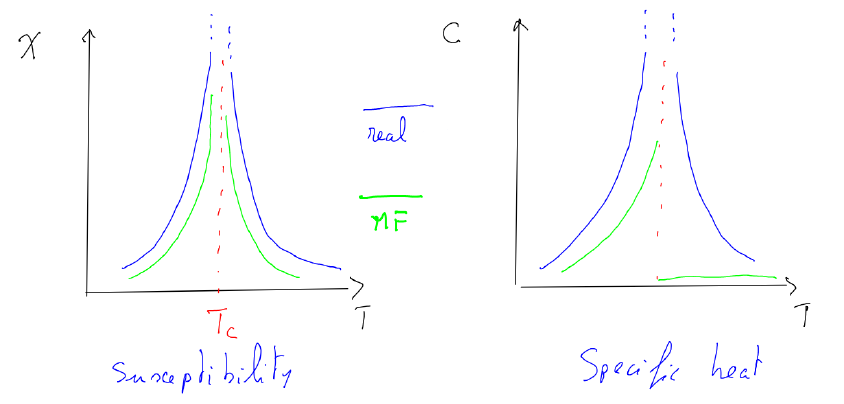
\includegraphics[width=0.9\textwidth]{\main/Images/chi-cv.png}
    \caption{Plot of the susceptibility $\chi$ (left) and the specific heat per node $c$ (right) as functions of temperature $T$. Both quantities \textit{diverge} for $T \to T_c$ in the real case - but this behaviour is captured by the mean field approximation only for $\chi$, and not for $c$ - for which only a \textit{finite} jump discontinuity is predicted. Even in the case of $\chi$, in a real system it diverges more rapidly than in the mean field model.}
    \label{fig:chi-cv}
\end{figure}

\section{Scaling ansatz\textit{s}}
We can use the power laws we have just found to write an \textbf{equation of state} connecting the external field $h$, the magnetization $m$ and distance to criticality $t$. 
We start from (\ref{eqn:h-eq}), highlight a $t$ and collect a $m^3$:
\begin{align*}
    h = m^3 \Bigg[\frac{1}{3} + \overbrace{\frac{K_c - K}{K_c}}^{t}m^{-2} + O(m^2) \Bigg] \qquad K \sim K_c;\> h\sim 0
\end{align*}
As in the mean-field $\beta = 1/2$ (\ref{eqn:m-power-law-h0}), we can rewrite $m^{-2} = m^{-1/\beta}$. We then use (\ref{eqn:m-power-law-h}) to write $m^3 = m|m|^{\delta-1}$, leading to the \textbf{scaling ansatz}, first conjectured by Widom in 1960:
\begin{align}\label{eqn:h-equation-state}
    h = m|m|^{\delta -1} h_s(t|m|^{-1/\beta}) \qquad  \quad t = \frac{T-T_c}{T_c}  
\end{align}
Where $h_s$ (the \q{scaling function}) has the following form in the mean field approximation:
\begin{align}
    h_s(x) = \frac{1}{3} + x
    \label{eqn:h-s-mean-field}
\end{align}
Expression (\ref{eqn:h-equation-state}) is certainly a valid relation between $h$, $m$ and $t$ near criticality in the mean field approximation - but we \textit{suppose}\footnote{That is why it is called an \textit{ansatz}.} that it holds in more general cases, perhaps with different choices of exponents $\beta, \delta$ or scaling function $h_s$. In particular, we make the hypothesis that $h_s$ \textit{should be \q{similar}} to (\ref{eqn:h-s-mean-field}), and in particular should be \textbf{non-decreasing} and vanishing at a \textbf{negative} point $x_0$  (fig. \ref{fig:scaling-function}).

\begin{figure}[H]
    \centering
    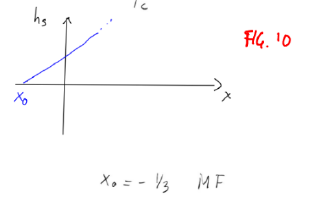
\includegraphics[width=0.7\textwidth]{\main/Images/scaling-function.png}
    \caption{Plot of the scaling function $h_S$ for the Mean Field case.}
    \label{fig:scaling-function}
\end{figure}

Equation (\ref{eqn:h-equation-state}) summarizes the previous scaling laws, in particular (\ref{eqn:m-power-law-h0}), (\ref{eqn:m-power-law-h}) and (\ref{eqn:susceptibility-power-law}) in all cases ($h=0$ or $h\neq 0$, $T < T_c$ or $T > T_c$). So, if we assume that an equation of state of the form (\ref{eqn:h-equation-state}) holds indeed in a more general case, and not only in the mean field approximation, we have a way to re-derive all the scaling laws.

\medskip

Explicitly, assuming $h_S$ monotonically increasing with $h_S(x_0) = 0$ and $x_0 < 0$:
\begin{enumerate}
    \item \textbf{Magnetization}. If $h=0$, equation (\ref{eqn:h-equation-state}) becomes:
    \begin{align*}
        0 = m|m|^{\delta-1} h_s(t|m|^{-1/\beta})
    \end{align*}
    The possible solutions are $m=0$ or $t|m|^{-1/\beta} = x_0 < 0$. The second one is acceptable only if $t < 0$, and in that case:
    \begin{align*}
        -|t| |m|^{-1/\beta} = -|x_0| \Rightarrow |m| = \left|\frac{t}{x_0}  \right|^{\beta}
    \end{align*}
    
    However, the second one is present only if $t < 0$, and so:
    \begin{align}
        m = \begin{cases}
            0 & t > 0\\
            |t|^\beta/|x_0|^\beta & t < 0
        \end{cases}%Different from the notes
        \label{eqn:magnetization-rules}
    \end{align} 
    In the mean field, $\beta = 1/2$ and $x_0=-1/3$, and so (\ref{eqn:magnetization-rules}) is equivalent to (\ref{eqn:m-power-law-h0}). 
    \item \textbf{Susceptibility}. Differentiating (\ref{eqn:h-equation-state}) with respect to $m$ and evaluating at $h=0$ leads to:
    \begin{align*}
        \chi^{-1}(h=0) &= \pdv{h}{m}\Big|_{h=0} \underset{(\ref{eqn:h-equation-state})}{=} \delta |m|^{\delta - 1} h_S(\underbrace{ t|m|^{-1/\beta}}_{x}) +\cancel{ m}|m|^{\delta-1}h_S'(t|m|^{-1/\beta})\frac{t|m|^{-1/\beta}}{\cancel{m}} \left(-\frac{1}{\beta} \right) = \\
        &=|m|^{\delta-1}\left[\delta h_S(x) - \frac{x}{\beta} h_S'(x) \right]_{h=0} \qquad x \equiv t|m|^{-1/\beta}
    \end{align*}
    
    For $t < 0$, the scaling is given by:
    \begin{align*}
        \chi^{-1} \propto |m|^{\delta-1} \underset{(\ref{eqn:magnetization-rules})}{\propto} |t|^{\beta (\delta-1)} = |t|^{\gamma_-} \qquad \gamma_- \equiv \beta(\delta-1)
    \end{align*}
    In the mean field, $\beta = 1/2$ and $\delta=3$, and so $\gamma_- = 1$, and $\chi \propto |t|^{-1}$, which is the same result we got in (\ref{eqn:susceptibility-power-law}).

    %At high temperature ($T > T_c$, $t > 0$) instead, we expect thermal noise to dominate, making the spins \q{independent}, and so $m = \tanh \sim h$ for $m \approx 0$, meaning that $m \approx h$ and $x \gg 1$. %TODO Finish last part of pag. 20
\end{enumerate}

In essence, the scaling ansatz (\ref{eqn:h-equation-state}) comes from the peculiar scaling of $m$ in a neighbourhood of criticality (fig. \ref{fig:criticality-vicinity}), and in particular: 
\begin{enumerate}[label=\alph*)]
    \item \label{item:1} For $h=0$ fixed and $t = (T-T_c)/T_c \approx 0$ (i.e. varying in the vicinity of the critical point), $m \propto (-t)^\beta$ for $t \lesssim 0$ (\ref{eqn:m-power-law-h0}).
    \item \label{item:2} For $t=0$ fixed and $h$ varying, $|m| \propto |h|^{1/\delta}$ (\ref{eqn:m-power-law-h}).
\end{enumerate} 

\begin{figure}[H]
    \centering
    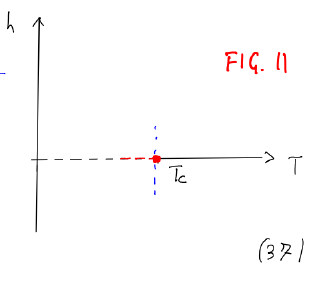
\includegraphics[width=0.6\textwidth]{\main/Images/criticality-vicinity.png}
    \caption{Phase diagram in $h$ and $T$. Singularities of $F_V$ are represented as the black dots at the left of $T_c$. The scaling ansatz describes how $m$ changes when approaching the critical point \textit{horizontally} (along the red path), i.e. at $h=0$ and varying $T$, or \textit{vertically}, i.e. at $T = T_c$ and varying $h$.}
    \label{fig:criticality-vicinity}
\end{figure}

In principle it is natural to say that $h$ should depend on two independent variables - $t$ and $m$ - but the choice of the \textit{form} of (\ref{eqn:h-equation-state}) arises from some \textbf{non-trivial} dimensional analysis arguments. The idea comes from observing that certain \textit{ratios} of quantities - due to their scaling behaviour near criticality (\ref{item:1} and \ref{item:2}) - are \q{dimensionless}\footnote{Not in the sense that being \textit{pure numbers}, i.e. not having physical dimensions (e.g. $\si{\kilo\g}$, $\si{T}$, $\si{\K}$ etc.) - which is a matter of the so-called na\"ive dimensional analysis. The \q{non-trivial} dimensional analysis deals with \textit{scaling} and \textit{local behaviours}.}, in the sense that, near criticality, they \textit{do not depend} anymore on the distance from the critical point and are \q{devoid} of singularities. Some of them are $h/m|m|^{\delta-1}$, $t/|m|^{1/\beta}$ and $t|h|^{-1/\delta \beta}$ - and so (\ref{eqn:h-equation-state}) is written as a function of such arguments.


\begin{figure}[H]
    \centering
    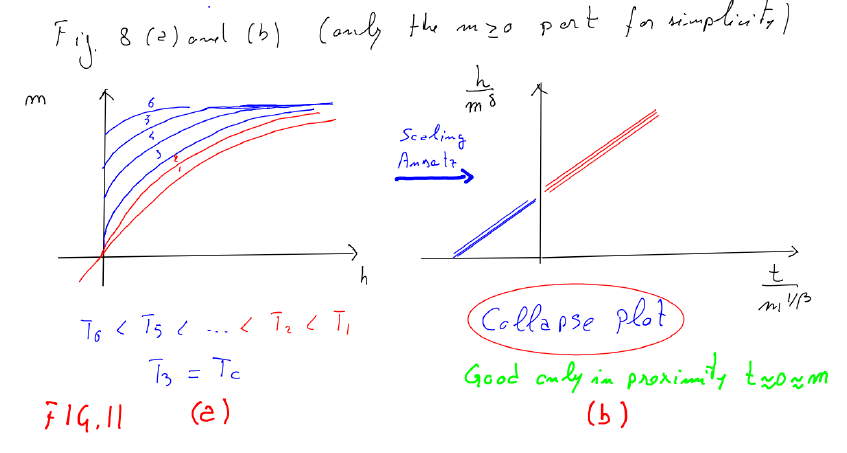
\includegraphics[width=0.9\textwidth]{\main/Images/collapse_plot.png}
    \caption{(a): $m(h)$ for different values of $K(T)$. When $T > T_c$ (hot system), $m(h)$ passes through the origin (red lines), while if $T < T_c$ (cold system), there is a nonzero spontaneous magnetization, i.e. $m(0) \neq 0$. As $m(h)$ is an odd function, only the first quadrant is shown for simplicity. If we instead plot \q{dimensionless} variables (b), all these curves \textit{collapse} into a single line (at least for $K(T)$ close to $K_c = K(T_c)$, i.e. $t \approx 0 \approx m$). This happens in the mean field approximation, and motivates a generalization to more complex systems giving rise to the scaling ansatz (\ref{eqn:h-equation-state}).}
    \label{fig:collapse_plot}
\end{figure}

\subsection{Two-point correlation function}
By shining a light on a fluid and measuring its scattering we can estimate how the density (and thus the refraction index) changes from point to point, and in particular its \textit{correlation} between different points. That's why it is important to compute correlation functions, especially the \textbf{two-point correlation} one:
\begin{align*}
    g(\bm{r}) \equiv \langle \sigma_x \sigma_y \rangle - \langle \sigma_x \rangle \langle \sigma_y \rangle
\end{align*} 

\subsubsection{Ising Model in $d=1$}
Before computing $g(\bm{r})$ in a generic dimension using the mean field model, we study a simpler case - namely, the $d=1$ IM with $h=0$ and \textbf{open boundary} conditions. 

We previously obtained:
\begin{align}\label{eqn:zeromean}
    \langle \sigma_x \rangle &\underset{(\ref{eqn:symmetry-arg}, \text{ pag.} \pageref{eqn:symmetry-arg})}{=}  0
\end{align}
For the correlation, we proceed by explicitly computing the average:
\begin{align*}
    \langle \sigma_x \sigma_y \rangle &= \sum_{\bm{\sigma}} \sigma_x \sigma_y \frac{1}{Z}  \exp\left(K \sum_z \sigma_z \sigma_{z+1}\right) =\\
    \shortintertext{Factoring the exponential over neighbouring pairs:}
    &= \sum_{\bm{\sigma}} \sigma_x \sigma_y \frac{1}{Z}  \prod_z \hlc{Yellow}{\exp\left(K \sigma_z \sigma_{z+1} \right)} =
    \shortintertext{As $\sigma_z \sigma_{z+1}$ is a binary variable (it can be only $\pm 1$), we can rewrite it using (\ref{eqn:ehsigma}, pag. \pageref{eqn:ehsigma}):}
    &= \sum_{\bm{\sigma}} \frac{\sigma_x \sigma_y}{Z}  \prod_z  (\cosh K + \sigma_z \sigma_{z+1} \sinh K)
    \shortintertext{Then we expand $Z = (2\cosh K)^N$ (\ref{eqn:Z-open-boundaries}, pag. \pageref{eqn:Z-open-boundaries}) and simplify the $\cosh K$:}
    &= \sum_{\bm{\sigma}} \sigma_x \sigma_y \frac{\displaystyle \prod_z \cosh K (1+ \sigma_z \sigma_{z+1} \tanh K)}{(2\cosh K)^L} = \\
    &= \sum_{\bm{\sigma}} \sigma_x \sigma_y \frac{\displaystyle \cancel{(\cosh K)^N} \prod_z (1+\sigma_z \sigma_{z+1} \tanh K)}{(2\cancel{\cosh K})^N} =\\
    &= \frac{1}{2^N} 
    \sum_{\bm{\sigma}} \sigma_x \sigma_y \prod_z (1 + \sigma_z \sigma_{z+1} \tanh K) 
\end{align*}
To proceed, let's denote $\tanh K \equiv A$ for simplicity, and expand both the sum and the product, assuming $x < y$:
\begin{align*}
    &= \frac{1}{2^N} \sum_{\sigma_1 = \pm 1} \cdots \sum_{\sigma_N = \pm 1} \sigma_x \sigma_y (1+\sigma_1 \sigma_2A) \cdots (1+\sigma_{x-1}\sigma_xA) \cdots (1+\sigma_{y-1}\sigma_yA) \cdots(1+ \sigma_{N-1}\sigma_NA) \span
    \shortintertext{We can \textit{factor out} all elements except the last, and perform the sum over $\sigma_{N}$:}
    &=\frac{1}{2^N}\left[\sum_{\sigma_1 = \pm 1} \cdots \sum_{\sigma_{N-1} = \pm 1}
    \sigma_x \sigma_y(1+\sigma_1 \sigma_2 A)\cdots(1+\sigma_{N-2}\sigma_{N-1}) 
    \right] \left[\sum_{\sigma_N = \pm 1} (1+\sigma_{N-1} \sigma_N A)\right] \span
\end{align*}
Note that:
\begin{align*}
    \sum_{\sigma_N = \pm 1} (1+\sigma_{N-1} \sigma_N A ) = 1 +\cancel{ \sigma_{N-1} A }+1 - \cancel{\sigma_{N-1} A} = 2
\end{align*}
Leading to:
\begin{align*}
    =\frac{1}{2^N} \sum_{\sigma_1 = \pm 1} \cdots \sum_{\sigma_{N-1} = \pm 1}
    \sigma_x \sigma_y(1+\sigma_1 \sigma_2 A)\cdots(1+\sigma_{N-2}\sigma_{N-1}A) \cdot 2
\end{align*}
We can then sum over $\sigma_{N-1}$, which will result in another factor $2$, and reiterate until we arrive at the sum over $\sigma_y$:
\begin{align*}
    =\frac{1}{2^N} \sum_{\sigma_1=\pm 1} \cdots \sum_{\sigma_y = \pm 1} \sigma_x (1+ \sigma_1 \sigma_2 A) \cdots  \sigma_y(1+\sigma_{y-1} \sigma_yA) \cdot 2^{N-y}
\end{align*}
If we now compute the sum over $\sigma_y$, the result will be different due to the added factor:
\begin{align*}
    \sum_{\sigma_y = \pm 1} \sigma_y(1+\sigma_{y-1} \sigma_yA) = 1 + \sigma_{y-1}A \textcolor{Red}{-}(1 - \sigma_{y-1}A) = 2 \sigma_{y-1}A
\end{align*}
Beside the usual factor $2$, now we have also a factor $A$ and a $\sigma_{y-1}$:
\begin{align*}
    =\frac{1}{2^N} \sum_{\sigma_1 = \pm 1} \cdots \sum_{\sigma_{y-1} = \pm 1} \sigma_x (1+\sigma_1 \sigma_2 A) \cdots \sigma_{y-1} (1+\sigma_{y-2}\sigma_{y-1}A) \cdot 2^{N-y+1} A 
\end{align*}
Due to the added $\sigma_{y-1}$, also the \textit{next} sum will produce (beside the $2$) also an $A$ and a $\sigma_{y-2}$, and so on. This continues until we arrive at the sum over $\sigma_x$:
\begin{align*}
    = \frac{1}{2^N} \sum_{\sigma_1=\pm 1} \cdots \sum_{\sigma_x = \pm 1} (1+\sigma_1 \sigma_2 A) \cdots \sigma_x^2(1+\sigma_{x-1}\sigma_xA) \cdot 2^{N-x} A^{y-x}
\end{align*} 
Note the $\sigma_x^2$: one $\sigma_x$ was there from the start, the other was produced by summing over $\sigma_{x+1}$. However, as $\sigma_x = \pm 1$, $\sigma_x^2 \equiv 1$ in any case, thus making the sum \q{go back to normal}:
\begin{align*}
    \sum_{\sigma_x = \pm 1} \underbrace{\sigma_x^2}_{1} (1+\sigma_{x-1}\sigma_xA) = 1 + \cancel{\sigma_{x-1}A} + 1 - \cancel{\sigma_{x-1}A} = 2
\end{align*}
From now on, all the remaining sums will just produce a factor $2$ each, and nothing more. So, at the end:
\begin{align*}
    \langle \sigma_x \sigma_y \rangle = \frac{1}{\cancel{2^N}} A^{y-x} \cancel{2^N} = (\tanh K)^{y-x}
\end{align*}
Here we supposed $x < y$. If $y < x$ instead, nothing really changes in the argument apart from the sign of the exponent. So, in general, we may write:
\begin{align}\label{eqn:xy-correlation}
    \langle \sigma_x \sigma_y \rangle = (\tanh K)^{|y-x|}
\end{align}
Denoting with $r = |y-x|$ the \textbf{distance} between the \textit{two points} $x$ and $y$, we can finally compute the correlation function $g(r)$, and rewrite it as an exponential:
\begin{align}\label{eqn:2point-exp-behaviour}
    g(r) = \underbrace{\langle \sigma_x \sigma_y \rangle}_{(\ref{eqn:xy-correlation})}  - \underbrace{\langle \sigma_x \rangle \langle \sigma_y \rangle}_{0\>(\ref{eqn:zeromean})} = (\tanh K)^{|r|} \equiv \exp\left(-\frac{|r|}{\xi(K)} \right)
\end{align}
where $\xi(K)$ is called the \textbf{correlation length}, and measures the \textit{decay} of correlations. In other words, spins are significantly correlated only when they are $|r| < \xi(K)$ positions apart. 

\medskip

Note that:
\begin{align*}
    \xi(K) = - \frac{1}{\ln \tanh K}  
\end{align*}
diverges when $K \to \infty$, i.e. when $T \to 0$. At very low temperature, the one-dimensional Ising model becomes \textit{fixed} in a extremely correlated configuration - as if $T=0$ were its the \textbf{critical temperature}. Still, note that this does not agree with the mean field model, for which $K_c = 1/2d = 1/2 \Rightarrow T_c = 2 J /k_B$. 

\medskip

The divergence of the correlation length $\xi(K)$ is fundamental for \textbf{universality}: as all microscopical parts of the system can interact with the \textit{whole} system, the \q{exact specifics} do not matter anymore, but only the most \textit{fundamental} characteristics of the system.

\subsubsection{General case: the correlation ansatz}
The exponential behaviour of the two-point correlation function (\ref{eqn:2point-exp-behaviour}) motivates an \textit{ansatz} for models in $d \geq 2$. More precisely, when $t \neq 0$ (i.e. $T \neq T_c$) the two-point correlation function is hypothesized to have the form:\marginpar{\vspace{3em}Correlation ansatz}
\begin{align}\label{eqn:corr-ansatz-t}
    g(\bm{r}, t) = r^{-\tau} \exp\left(-\frac{\tau}{\xi(t)} \right) \qquad r=\norm{\bm{r}}
\end{align} 
with the correlation length diverging near the critical point:
\begin{align}\label{eqn:corr-length-t}
    \xi(t) = C_\pm |t|^{-\nu} \qquad t \approx 0, \> h = 0
\end{align}
for some proper choices of parameters $\tau$, $\nu$ and $C_\pm$. In more general cases, $\xi(t)$ may also depend (weakly) on the \textit{direction} of $\bm{r}$, meaning that the system is not isotropous.

\medskip

At the critical point $t = (T-T_c)/T_c = 0$, with $h=0$, the correlation \textit{does not diverge} anymore, but it's described instead by a power law: \marginpar{\vspace{1em}Correlation ansatz at $t=0$}
\begin{align}
    g(\bm{r}, t) \sim \norm{\bm{r}}^{-(d-2 + \eta)}\label{eqn:corr-ansatz-t0}
\end{align}
where the added exponent $\eta$ is called the \textbf{anomalous dimension}\index{Anomalous dimension}. 

\medskip

We can combine (\ref{eqn:corr-ansatz-t}) and (\ref{eqn:corr-ansatz-t0}) by writing an \textit{equation of state} for the correlation length $\xi(K)$, as a function of the only two \q{dimensionless} scaling variable $r/\xi$ and $t |h|^{-1/\beta \delta}$:
\begin{align}\label{eqn:corr-length-ansatz}
    \xi(t, h) = |t|^{-\nu} \hat{\xi} (t |h|^{-1/\beta \delta})
\end{align}
leading to the \textbf{complete} ansatz for the two-point correlation ansatz:\marginpar{\vspace{1em}The \q{complete} correlation ansatz}
\begin{align}\label{eqn:correlation-ansatz-full}
    g(\bm{r}, t, h) = r^{-(d-2+\eta)} \tilde{g} \left(\frac{r}{\xi}, t h^{-1/\beta \delta} \right)
\end{align} 

Before proceeding, we note that (\ref{eqn:correlation-ansatz-full}) leads to an interesting relation between $\gamma$ (the exponent defining the scaling for the susceptibility) and $\eta, \delta$, i.e. the exponents appearing in the correlation ansatz.

\medskip

Recall the fluctuation dissipation theorem (\ref{eqn:fluctuation_dissipation}, \pageref{eqn:fluctuation_dissipation}):
\begin{align*}
    \chi &= \pdv{h} \langle \frac{\sum_x \sigma_x}{N}  \rangle = \frac{1}{N}[ \langle \sum_{xy} \sigma_x \sigma_y \rangle - \langle \sum_x \sigma_x \rangle^2]  =\\
    &= \frac{1}{N} \sum_{xy} \Big(\underbrace{\langle \sigma_x \sigma_y \rangle - \langle \sigma_x \rangle \langle \sigma_y \rangle}_{g(x-y, t, h)} \Big) = \sum_{\bm{r}} g(\bm{r}, t, h) 
\end{align*}
At $h=0$ and $t\approx 0$, $\tilde{g}$ varies slowly, because it is defined as a function of \q{dimensionless} variables. So we can consider the continuum limit, and substitute the sum over $\bm{r}$ with an integral:
\begin{align*}
    \chi &= \int \dd[d]{\bm{r}} \tilde{g}\left(\frac{r}{\xi} \right) r^{-(d-2+\eta)} \underset{\bm{r}/\xi = \bm{x}}{=} \xi^{2-\eta} \underbrace{\int \dd[d]{\bm{x}} \tilde{g}(\bm{x}) x^{-(d-2+\eta)}}_{\text{Constant in $h$, $t$}} =\\
    &= \xi^{2- \eta} \cdot \text{Const.} \underset{(\ref{eqn:corr-length-t})}{\propto} |t|^{-\nu(2-\eta)}  
\end{align*}
and comparing with (\ref{eqn:susceptibility-power-law}) leads to the following \textbf{scaling relation}:
\begin{align}\label{eqn:scaling-relation}
    \gamma = \nu (2 - \eta)
\end{align} %TODO Do the computation

\subsection{Hyperscaling}
Finally, we proceed yet further in finding new ansatz\textit{s}. 

In the previous section, we found that the correlation length $\xi$ can be regarded as new scale length that emerges spontaneously near criticality. 

So, na\"ively we know that the free energy \textbf{density} $f$ scales as $L^{-d}$, where $L$ is the physical length scale of the system and $d$ its dimension. However, near criticality, we may \textit{guess} that the \q{most important} length scale becomes instead $\xi$, leading to the ansatz:
\begin{align*}
    f(T, h=0) = \frac{F(T, h=0)}{N} = \xi^{-d} \cdot \text{Const.} + \text{Less Singular Terms} 
\end{align*} 
As $\xi \sim |t|^{-\nu}$ (\ref{eqn:corr-length-ansatz}), then, near criticality:
\begin{align*}
    f(T, h=0) \sim |t|^{d \nu}
\end{align*}
Differentiating two times with respect to $T$ we can derive a similar relation for the heat capacity:
\begin{align*}
    C = - T \pdv[2]{T} F(T, h=0) &= \text{Const} \cdot |t|^{d \nu - 2} + \text{l.s.t} 
\end{align*}
Comparing with (\ref{eqn:specific-heat-power-law}), we find a relation for the exponent $\alpha$, known as the \textbf{hyper-scaling relation} :
\begin{align}\label{eqn:hyper-scaling-relation}
    \alpha = 2 - d \nu
\end{align}
The \textit{hyper} comes from the fact that (\ref{eqn:hyper-scaling-relation}) is the only relation thus far that \textit{explicitly} involves the dimension $d$ of the system. Moreover, it is known to hold only below some \textbf{critical dimension} $d_U$ (the \q{upper} dimension), and violated in $d > d_U$. In case of the Ising Model, $d_U = 4$.


\subsection{Summary of scaling relations}
We have introduced a total of $6$ exponents:
\begin{enumerate}
    \item $\beta$, regulating the magnetization $m$ as a function of temperature (\ref{eqn:magnetization-rules})
    \item $\gamma$, for the susceptibility $\chi$ as a function of temperature (\ref{eqn:susceptibility-power-law})
    \item $\delta$, regulating the magnetization $m$ as a function of the magnetic field $h$ (\ref{eqn:m-power-law-h})
    \item $\alpha$, for the specific heat $c$ versus temperature (\ref{eqn:specific-heat-power-law})
    \item $\eta$, dealing with the \textit{decay} of the two-point correlation function near the critical point as a function of the distance $t$ from it (\ref{eqn:correlation-ansatz-full})
    \item $\nu$, describing the divergence of the correlation length near criticality as a function of $t$ (\ref{eqn:corr-length-ansatz})
\end{enumerate}
and $4$ scaling relations between them:
\begin{subequations}\label{eqn:scaling-relations}
    \begin{align}
        \beta (\delta - 1) &= \gamma\\
        \nu(2- \eta) &= \gamma\\
        \beta ( \delta + 1) &= 2 - \alpha\\
        d \nu -2 &= \alpha
    \end{align}
\end{subequations}
meaning that, at the end, only $2$ exponents are independent.

%TODO Add footnote pag. 24 in a appr box


\end{document}
